\documentclass{article}
\usepackage{arxiv}

\usepackage[utf8]{inputenc}
\usepackage[english, russian]{babel}
\usepackage[T1]{fontenc}
\usepackage{url}
\usepackage{booktabs}
\usepackage{amsfonts}
\usepackage{nicefrac}
\usepackage{microtype}
\usepackage{bm}
\usepackage{lipsum}
\usepackage{graphicx}
\usepackage{natbib}
\usepackage{doi}
\usepackage{mathtools}


\newcommand{\argmin}{\arg\!\min}
\newcommand{\argmax}{\arg\!\max}


\title{Автоматическая регуляризации байесовских нейронных сетей}

\author{
    Басов Дмитрий Константинович
}
\date{}

\renewcommand{\shorttitle}{Автоматическая регуляризации байесовских нейронных сетей}

\begin{document}
    \maketitle

    \begin{abstract}
        В байесовском выводе, в отличии от гипотезы максимального правдоподобия,
        не делается никаких предположений о размере обучающей выборки.
        Это делает байесовские модели устойчивыми к переобучению.

        Однако применение байесовского вывода сопряжено со следующими проблемами:
        заданием подходящего априорного распределения и вычислением апостериорного распределения весов модели.

        В данной работе предлагается следующее решение этих проблем:
        \begin{enumerate}
            \item Применяя вариационный вывод,
                апостериорное распределение весов модели аппроксимируется
                нормальным распределением с диагональной матрицей ковариации,
                и задача сводится к максимизации нижней вариационной границы.
                В этом случае каждый вес модели определяется двумя обучаемыми параметрами.
            \item Априорное распределение весов модели задается в виде
                нормального распределения с нулевым матожиданием
                и диагональной матрицей ковариации, элементы которой вычисляется из данных.
                Этот приём лежит в основе Relevance Vector Machine~--- байесовского варианта SVM.
        \end{enumerate}

        Полученную модель можно рассматривать как
        ансамбль из бесконечного числа нейронных сетей,
        веса которых сэмплируются из нормального распределения.
        При этом каждый вес имеет свой индивидуальный коэффициент $L2$ регуляризации,
        который автоматически определяется из тренировочных данных при обучении.

    \end{abstract}

    \section{Обозначения и сокращения}
    $\pmb{x} \odot \pmb{y}$ --- поэлементное произведение (произведение Адамара) векторов \par
    $\mathcal{L}$ --- Evidence Lower Bound (ELBO) \par
    $
        KL(q \parallel p)
        =
        \int_{}{
            q(\pmb{Z})
            \,
            \ln{
                \frac
                    {q(\pmb{Z})}
                    {p(\pmb{Z})}
            }
            \,
            d\pmb{Z}
        }
    $ --- дивергенция Кульбака--Лейблера \par
    $\pmb{x}$ --- вектор признаков \par
    $\pmb{y}$ --- вектор целевой переменной \par
    $D$ --- датасет --- пары значений $\{\pmb{x_i}$, $\pmb{y_i}\}$, где $i = 1, \dots, L$ \par
    $\pmb{W}$ --- веса модели --- случайная величина размерности M \par
    $p(\pmb{y} | \pmb{x}, D)$ --- предсказательное распределение \par
    $
        p(D | \pmb{W})
        =
        \prod_{i=1}^{L}{
            p(\pmb{y_i} | \pmb{x_i}, \pmb{W})
        }
    $ — правдоподобие (likelihood) \par
    $p(\pmb{W})$ --- априорное распределение весов модели (prior) \par
    $p(\pmb{W}| D)$ --- апостериорное распределение весов модели (posterior) \par
    $q_{\pmb{\theta}}(\pmb{W})$ --- аппроксимация апостериорного распределения весов модели \par
    $\pmb{\theta}$ --- обучаемые параметры байесовской модели \par

    \section{Введение}

    В классическом машинном обучении делается следующее предположение:
    веса модели $\pmb{W}$ являются пусть и неизвестной, но фиксированной величиной.
    В этом случае можно получить точечную оценку весов модели согласно гипотезе максимального правдоподобия.
    \[
        \pmb{W_{ML}} = \argmax_{\pmb{W}} p(D | \pmb{W})
    \]
    Тогда распределение $p(\pmb{y} | \pmb{x}, D)$ аппроксимируется следующим образом:
    \[
        p(\pmb{y} | \pmb{x}, D) \approx p(\pmb{y} | \pmb{x}, \pmb{W_{ML}})
    \]
    Однако это справедливо при условии, что количество объектов в датасете D
    сильно больше количества весов модели ($L \gg M$).
    Если это не так, веса модели $\pmb{W}$ могут слишком сильно подстроиться
    под обучающую выборку D, что черевато переобучением.

    Для борьбы с переобучением используется ряд приёмов (штрафы на норму весов, early stopping, dropout),
    однако для их настройки требуются вычислительные ресурсы и отложенные
    (не участвующие в обучении) выборки данных.

    Альтернативным подходом к машинному обучению является нахождение апостериорного распределения весов модели $p(\pmb{W}| D)$ по теореме Байеса.
    \[
        p(\pmb{W}| D)
        =
        \frac
            {
                p(D | \pmb{W})
                \,
                p(\pmb{W})
            }
            {
                \int{
                    p(D | \pmb{W})
                    \,
                    p(\pmb{W})
                    \,
                    d\pmb{W}
                }
            }
    \]
    Тогда предсказательное распределение $p(\pmb{y} | \pmb{x}, D)$ рассчитывается следующим образом:
    \[
        p(\pmb{y} | \pmb{x}, D)
        =
        \int{
            p(\pmb{y} | \pmb{x}, \pmb{W})
            \,
            p(\pmb{W} | D)
            \,
            d\pmb{W}
        }
    \]
    Байесовские модели можно рассматривать как ансамбль из бесконечного числа моделей,
    веса которых сэмплируются из распределения
    $p(\pmb{W}| D)$.
    Такой подход устойчив к переобучению, так как о размере обучающей выборки не делается никаких предположений.
    Однако возникают следующие проблемы: выбор подходящего априорного распределения
    $p(\pmb{W})$
    и вычисление апостериорного распределения
    $p(\pmb{W}| D)$.

    Неудачный выбор $p(\pmb{W})$ может сильно ухудшить качество модели,
    а расчёт апостериорного распределения $p(\pmb{W}| D)$
    требует вычисления интеграла по всему пространству весов модели,
    что для нейронных сетей практически невозможно.

    В данной статье предлагается следующий подход к решению этих проблем.

    \begin{enumerate}
        \item Применяя вариационный вывод, распределение $p(\pmb{W}| D)$
            аппроксимируется распределением $q_{\pmb{\theta}}(\pmb{W})$,
            и задача сводится к максимизации нижней вариационной границы
            $\mathcal{L}$ по параметрам $\pmb{\theta}$.
        \item Распределение $q_{\pmb{\theta}}(\pmb{W})$
            задаётся в виде нормального распределения с диагональной матрицей ковариации.
%             То есть каждый вес модели определяется двумя числами,
%             которые определяют его математическое ожидание и дисперсию.
%             Таким образом, количество обучаемых параметров
%             относительно классической нейронной сети возрастает в 2 раза.
        \item Так как распределение $q_{\pmb{\theta}}(\pmb{W})$
            является нормальным, применяя трюк с репараметризацией,
            становится возможным использовать градиентные методы
            для максимизации $\mathcal{L}$.
        \item Априорное распределение весов модели $p(\pmb{W})$
            задаётся в виде нормального распределения с нулевым матожиданием
            и диагональной матрицей ковариации, элементы которой определяются при обучении из датасета D.
            Такой подход обладает большой универсальностью,
            однако из--за этого теряется теоретическая устойчивость к переобучению.
            Идея определения некоторых параметров априорного распределения
            $p(\pmb{W})$ из датасета D
            известна как эмпирический Байес.
        \item Вводятся новые параметры $\pmb{\gamma}$ и $\pmb{\rho}$,
            через которые выражаются матожидание и дисперсия распределения
            $q_{\pmb{\theta}}(\pmb{W})$.
            Это нужно, чтобы избежать неопределенности деления $\frac{0}{0}$,
            которая может возникнуть из--за определения дисперсии распределения $p(\pmb{W})$ из данных.
    \end{enumerate}

    \section{Постановка задачи}

    Задача машинного обучения с учителем
    в вероятностной постановке формулируется следующим образом: получить
    распределение вероятностей $p(\pmb{y} | \pmb{x}, D)$
    целевой переменной $\pmb{y}$
    для неразмеченных $\pmb{x}$, используя информацию из датасета D.
    В случае параметрических моделей, которыми являются нейронные сети,
    информация из датасета D кодируется посредством весов модели $\pmb{W}$.
    Сделаем следующие преобразования:
    \[
        p(\pmb{y} | \pmb{x}, D)
        =
        \int_{}{
            p(\pmb{y}, \pmb{W} | \pmb{x}, D)
            \,
            d\pmb{W}
        }
        =
        \int_{}{
            p(\pmb{y} | \pmb{W}, \pmb{x}, D)
            \,
            p(\pmb{W} | \pmb{x}, D)
            \,
            d\pmb{W}
        }
        =
        \int_{}{
            p(\pmb{y} | \pmb{W}, \pmb{x})
            \,
            p(\pmb{W} | D)
            \,
            d\pmb{W}
        }
    \]

    Пояснения:
    \begin{itemize}
    \item
        $
            p(\pmb{y} | \pmb{x}, D)
            =
            \int_{}{
                p(\pmb{y}, \pmb{W} | \pmb{x}, D)
                \,
                d\pmb{W}
            }
        $
        , так как для любых случайных величин
        $\pmb{a}$ и $\pmb{b}$ справедливо
        $
            p(\pmb{a})
            =
            \int{
                p(\pmb{a}, \pmb{b})
                \,
                d\pmb{b}
            }
        $
    \item
        $
            p(\pmb{y}, \pmb{W} | \pmb{x}, D)
            =
            p(\pmb{y} | \pmb{W}, \pmb{x}, D)
            \,
            p(\pmb{W} | \pmb{x}, D)
        $, так как для любых случайных величин $\pmb{a}$ и $\pmb{b}$ справедливо
        $
            p(\pmb{a}, \pmb{b})
            =
            p(\pmb{a}| \pmb{b})
            \,
            p(\pmb{b})
        $
    \item
        $
            p(\pmb{y} | \pmb{W}, \pmb{x}, D)
            =
            p(\pmb{y} | \pmb{W}, \pmb{x})
        $, так как вся информация из датасета D отражена в весах $\pmb{W}$
    \item
        $
            p(\pmb{W} | \pmb{x}, D)
            =
            p(\pmb{W} | D)
        $, так как веса модели $\pmb{W}$ не зависят от неразмеченных
        $\pmb{x}$, которых не было в датасете D.
    \end{itemize}

    Получим выражение для $p(\pmb{W}| D)$, используя формулу Байеса:
    \[
        p(\pmb{W}| D)
        =
        \frac
            {p(\pmb{W}, D)}
            {p(D)}
        =
        \frac
            {p(\pmb{W}, D)}
            {
                \int{
                    p(\pmb{W}, D)
                    \,
                    d\pmb{W}
                }
            }
        =
        \frac
            {
                p(D | \pmb{W})
                \,
                p(\pmb{W})
            }
            {
                \int{
                    p(D | \pmb{W})
                    \,
                    p(\pmb{W})
                    \,
                    d\pmb{W}
                }
            }
    \]

    Для аппроксимации распределения ответов модели можно воспользоваться методом Монте--Карло.
    Идея следующая: cэмплируем конечное количество весов
    $
        \pmb{
            \hat{W}_1
        }
        ,
        \dots
        ,
        \pmb{
            \hat{W}_T
        }
    $
    из распределения $p(\pmb{W}| D)$ и аппроксимируем распределение
    $p(\pmb{y} | \pmb{x}, D)$ следующим образом:
    \[
        p(\pmb{y} | \pmb{x}, D)
        \approx
        \frac{1}{T}
        \sum_{t=1}^{T}{
            p (
                \pmb{y} | \pmb{x},
                \pmb{\hat{W}_{t}}
            )
        }
    \]

    Однако для этого нужно иметь возможность сэмплировать из распределения $p(\pmb{W}| D)$.
    Получить аналитическое решение интеграла
    $
        \int {
            p(D | \pmb{W})
            \,
            p(\pmb{W})
            \,
            d\pmb{W}
        }
    $
    можно только в очень ограниченном числе случаев.

    Существует возможность сэмплировать из $p(\pmb{W}| D)$,
    используя методы Монте--Карло для марковских цепей (MCMC).
    Однако для больших датасетов и большого числа весов это практически невозможно.

    Альтернативным подходом к решению такой задачи является вариационный вывод~---
    аппроксимация распределения $p(\pmb{W}| D)$ распределением $q_{\pmb{\theta}}(\pmb{W})$,
    из которого сэмплировать намного проще.

    \section{Вариационный вывод}

    Идея вариационного вывода --- сведение задачи байесовского вывода к задаче максимизации нижней вариационной границы (ELBO) $\mathcal{L}$, которая для распределения $q_{\pmb{\theta}}(\pmb{W})$ записывается следующим образом:
    \[
    \mathcal{L} =
    \int_{}{} q_{\pmb{\theta}}(\pmb{W}) \cdot \ln{\dfrac{p(\pmb{W}, D)}{q_{\pmb{\theta}}(\pmb{W})}} d \pmb{W}
    \]

    Покажем мотивацию максимизации ELBO. Запишем выражение для $KL(q_{\pmb{\theta}}(\pmb{W})~||~p(\pmb{W}| D))$ и преобразуем его, используя тождество $p(\pmb{W}, D) = p(\pmb{W}| D)\cdot p(D)$:
    \[
    KL(q_{\pmb{\theta}}(\pmb{W})~||~p(\pmb{W}| D)) =
    \int_{}{} q_{\pmb{\theta}}(\pmb{W}) \cdot \ln{\dfrac{q_{\pmb{\theta}}(\pmb{W})}{p(\pmb{W}| D)}} d \pmb{W} =
    \int_{}{} q_{\pmb{\theta}}(\pmb{W}) \cdot \ln{\dfrac{p(D) \cdot q_{\pmb{\theta}}(\pmb{W})}{p(\pmb{W}, D)}} d \pmb{W} =
    \]\[
    \ln{p(D)} \cdot \int_{}{} q_{\pmb{\theta}}(\pmb{W}) d \pmb{W} - \int_{}{} q_{\pmb{\theta}}(\pmb{W}) \cdot \ln{\dfrac{p(\pmb{W}, D)}{q_{\pmb{\theta}}(\pmb{W})}} d \pmb{W} =
    \ln{p(D)} - \mathcal{L}
    \]

    Так как $\ln{p(D)}$ не зависит от $\pmb{\theta}$, максимизация $\mathcal{L}$ по параметрам $\pmb{\theta}$ ведёт к минимизации $KL(q_{\pmb{\theta}}(\pmb{W})~||~p(\pmb{W}| D))$. Тем самым, при максимизации $\mathcal{L}$ распределение $q_{\pmb{\theta}}(\pmb{W})$ будет приближаться к распределению $p(\pmb{W}| D)$.

    Преобразуем выражение для $\mathcal{L}$, используя тождество $p(\pmb{W}, D) = p(D | \pmb{W}) \cdot p(\pmb{W})$:
    \[
    \mathcal{L} =
    \int_{}{} q_{\pmb{\theta}}(\pmb{W}) \cdot \ln{\dfrac{p(\pmb{W}, D)}{q_{\pmb{\theta}}(\pmb{W})}} d \pmb{W} =
    \int_{}{} q_{\pmb{\theta}}(\pmb{W}) \cdot \ln{\dfrac{p(D | \pmb{W}) \cdot p(\pmb{W})}{q_{\pmb{\theta}}(\pmb{W})}} d \pmb{W} =
    \]\[
    \int_{}{} q_{\pmb{\theta}}(\pmb{W}) \cdot \ln{p(D | \pmb{W})} d \pmb{W} - \int_{}{} q_{\pmb{\theta}}(\pmb{W}) \cdot \ln{\dfrac{q_{\pmb{\theta}}(\pmb{W})}{p(\pmb{W})}} d \pmb{W} =
    \]\[
    \int_{}{} q_{\pmb{\theta}}(\pmb{W}) \cdot \ln{p(D | \pmb{W})} d \pmb{W} - KL(q_{\pmb{\theta}}(\pmb{W})~||~p(\pmb{W})) =
    \]\[
    \int_{}{} q_{\pmb{\theta}}(\pmb{W}) \cdot \sum_{i=1}^{L} {\ln{p(\pmb{y_{i}} | \pmb{x_{i}}, \pmb{W})}} d \pmb{W} - KL(q_{\pmb{\theta}}(\pmb{W})~||~p(\pmb{W}))
    \]

    Так как в случае нейронной сети аналитически посчитать интеграл по всему пространству весов $\pmb{W}$ не представляется возможным, воспользуемся следующей аппроксимацией для $p(\pmb{y} | \pmb{x}, D)$ и $\mathcal{L}$:
    \[
    p(\pmb{y} | \pmb{x}, D) \approx
    \int_{}{} p(\pmb{y} | \pmb{W}, \pmb{x}) \cdot q_{\pmb{\theta}}(\pmb{W}) d \pmb{W} \approx
    \dfrac{1}{T} \sum_{t=1}^{T}{p(\pmb{y} | \pmb{x}, \pmb{\hat{W}_{t}})}
    \]
    \[
    \mathcal{L} \approx
    \dfrac{1}{S} \sum_{j=1}^S \sum_{i=1}^{L} {\ln{p(\pmb{y_{i}} | \pmb{x_{i}}, \pmb{\hat{W}_{ij}})}} - KL(q_{\pmb{\theta}}(\pmb{W})~||~p(\pmb{W}))
    \]

    где $\pmb{\hat{W}_{t}}$ и $\pmb{\hat{W}_{ij}}$ --- сэмплы весов модели из распределения $q_{\pmb{\theta}}(\pmb{W})$.

    \section{Задание функциональных форм распределений}

    Для дальнейшнего вывода положим, что распределения $p(\pmb{W})$ и $q_{\pmb{\theta}}(\pmb{W})$ являются нормальными с диагональными матрицами ковариации:
    \[
    q_{\pmb{\theta}}(\pmb{W}) = N(\pmb{W} | \pmb{\mu}, diag(\pmb{\sigma_{q(\pmb{W})}})^{2})
    \]
    \[
    p(\pmb{W}) = N(\pmb{W} | \pmb{0}, diag(\pmb{\sigma_{p(\pmb{W})}})^{2})
    \]

    Так как распределение $q_{\pmb{\theta}}(\pmb{W})$ нормальное, мы можем использовать трюк с репараметризацией при сэмплировании весов, что позволяет использовать градиентные методы для оптимизации:
    $
    \pmb{\hat{W}_{ij}} = \pmb{\epsilon_{ij}}  \odot \pmb{\sigma_{q(\pmb{W})}} + \pmb{\mu}
    $, где $\pmb{\epsilon_{ij}}$ --- сэмпл из $N(\pmb{0}, \pmb{I})$.

    Так как распределения $p(\pmb{W})$ и $q_{\pmb{\theta}}(\pmb{W})$ нормальные, $KL(q_{\pmb{\theta}}(\pmb{W})~||~p(\pmb{W}))$ считается аналитически:
    \[
    KL(q_{\pmb{\theta}}(\pmb{W})~||~p(\pmb{W})) =
    \dfrac{1}{2}\sum_{k=1}^{M}(\dfrac{\sigma_{{q(W)_{k}}}^2}{\sigma_{{p(W)_{k}}}^2} + \dfrac{\mu_{k}^2}{\sigma_{{p(W)_{k}}}^2} - \ln{\dfrac{\sigma_{{q(W)_{k}}}^2}{\sigma_{{p(W)_{k}}}^2}} - 1)
    \]

    Априорное распределение весов модели $p(\pmb{W})$ имеет нулевое математическое ожидание (из соображений симметрии), и среднеквадратическое отклонение $\pmb{\sigma_{p(\pmb{W})}}$. В классическом байесовском выводе параметр $\pmb{\sigma_{p(\pmb{W})}}$ должен задаваться до начала обучения, то есть являться гиперпараметром. Однако мы можем воспользоваться техникой эмпирического Байеса, то есть определить параметр  априорного распределения $\pmb{\sigma_{p(\pmb{W})}}$ из данных.

    \section{Эмпирический Байес}
    Пусть $\pmb{\alpha} = diag(\pmb{\sigma_{p(\pmb{W})}})^{-2}$. Тогда выражение для $KL(q_{\pmb{\theta}}(\pmb{W})~||~p(\pmb{W}))$ будет иметь следующий вид:
    \[
    KL(q_{\pmb{\theta}}(\pmb{W})~||~p(\pmb{W})) =
    \dfrac{1}{2}\sum_{k=1}^{M}( \alpha_{k} \cdot \sigma_{{q(W)_{k}}}^2 + \alpha_{k} \cdot \mu_{k}^2 - (\ln{\sigma_{{q(W)_{k}}}^2} + \ln{\alpha_{k}}) - 1)
    \]

    Так как в выражении $\mathcal{L}$ интеграл $\int_{}{} q_{\pmb{\theta}}(\pmb{W}) \cdot \ln{p(D | \pmb{W})} d \pmb{W}$ не зависит от параметров распределения $p(\pmb{W})$, то:
    \[
    \dfrac{\partial \mathcal{L}}{\partial {\alpha_k}} =
    - \dfrac{\partial (KL(q_{\pmb{\theta}}(\pmb{W})~||~p(\pmb{W})))}{\partial {\alpha_k}} =
    -\dfrac{1}{2}(\sigma_{{q(W)_{k}}}^2 + \mu_{k}^2 - \dfrac{1}{\alpha_k}) =
    -\dfrac{1}{2}(\sigma_{{q(W)_{k}}}^2 + \mu_{k}^2 - \sigma_{{p(W)_{k}}}^2)
    \]

    Приравняв производную к нулю, получим:
    \[
    -\dfrac{1}{2}(\sigma_{{q(W)_{k}}}^2 + \mu_{k}^2 - \sigma_{{p(W)_{k}}}^2) = 0
    \]\[
    \sigma_{{p(W)_{k}}}^2 = \sigma_{{q(W)_{k}}}^2 + \mu_{k}^2
    \]

    Подставив полученное выражение для априорной дисперсии в $KL(q_{\pmb{\theta}}(\pmb{W})~||~p(\pmb{W}))$, получим:
    \[
    KL(q_{\pmb{\theta}}(\pmb{W})~||~p(\pmb{W})) =
    \dfrac{1}{2}\sum_{k=1}^{M}\ln({1 + \dfrac{\mu_{k}^2}{\sigma_{{q(W)_{k}}}^2}})
    \]

    Таким образом, мы свели задачу к максимизации $\mathcal{L}$ по параметрам $\pmb{\mu}$ и $\pmb{\sigma_{q(W)}}$.

    \section{Замена переменных}

    При максимизации $\mathcal{L}$ могут возникнуть ситуации, когда какой--либо вес модели перестает быть случайной величиной и вырождается в ноль ($\sigma_{{q(W)_{k}}} \rightarrow 0$ и $\mu_{k} \rightarrow 0$). Это приведет к неопределенности деления 0 на 0 при вычислении KL--дивергенции.

    Так же при градиентной оптимизации компоненты вектора $\pmb{\sigma_{q(\pmb{W})}}$ могут попасть в отрицательную область, что нежелательно, так как среднеквадратическое отклонение не может быть отрицательным по определению.

    Чтобы избежать этих проблем, сделаем следующую замену переменных:
    \[
    \pmb{\sigma_{q(\pmb{W})}} = \ln({1 + e^{\pmb{\rho}}}) = Softplus (\pmb{\rho})
    \]\[
    \pmb{\mu} = \pmb{\gamma} \odot \pmb{\sigma_{q(\pmb{W})}} = \pmb{\gamma} \odot Softplus (\pmb{\rho})
    \]

    Тогда:
    \[
    KL(q_{\pmb{\theta}}(\pmb{W})~||~p(\pmb{W})) =
    \dfrac{1}{2}\sum_{k=1}^{M}\ln({1 + \dfrac{\mu_{k}^2}{\sigma_{{q(W)_{k}}}^2}}) =
    \dfrac{1}{2}\sum_{k=1}^{M}\ln({1 + \gamma_{k}^{2}})
    \]

    Таким образом, задача сводится к минимизации следующей функции потерь по параметрам $\pmb{\rho}$ и $\pmb{\gamma}$:
    \[
    loss(\pmb{\rho}, \pmb{\gamma}) =
    - \dfrac{\mathcal{L}}{L} \approx
    -\dfrac{1}{S \cdot L} \sum_{j=1}^S \sum_{i=1}^{L}  {\ln{p(\pmb{y_{i}} | \pmb{x_{i}}, \pmb{\hat{W}_{ij}})}} + \dfrac{KL}{L}
    \]

    где:
    \[
    \pmb{\hat{W}_{ij}} = \pmb{\epsilon} \odot \pmb{\sigma} + \pmb{\mu}
    \]
    \[
    \pmb{\epsilon} \sim N(\pmb{0}, \pmb{I})
    \]
    \[
    \pmb{\sigma} = Softplus(\pmb{\rho})
    \]
    \[
    \pmb{\mu} = \pmb{\gamma} \odot \pmb{\sigma}
    \]
    \[
    KL = \dfrac{1}{2}\sum_{k=1}^{M}\ln({1 + \gamma_{k}^{2}})
    \]

    \section{Алгоритм обучения}

    Задаем шаг градиентного спуска $\alpha$ и инициализируем параметры распределения $q_{\pmb{\theta}}(\pmb{W})$ — $\pmb{\rho}$ и $\pmb{\gamma}$. Затем повторяем, пока не достигнем критерия остановки:
    \begin{enumerate}
        \item $\pmb{\sigma} \leftarrow Softplus(\pmb{\rho})$ --- расчёт среднеквадратических отклонений весов
        \item $\pmb{\mu} \leftarrow \pmb{\gamma} \odot \pmb{\sigma}$ --- расчёт математических ожиданий весов
        \item $\pmb{\epsilon} \leftarrow N(0, 1)$ --- сэмплирование случайных весов
        \item $\hat{\pmb{W}} \leftarrow \pmb{\epsilon} \odot \pmb{\sigma} + \pmb{\mu}$ --- репараметризация
        \item $nll \leftarrow -\dfrac{1}{L}\sum_{i=1}^{L}{\ln{p( \pmb{y_{i}} | \pmb{x_{i}}, \pmb{\hat{W}})}}$ --- расчёт среднего отрицательного логарифма правдоподобия (возможна аппроксимация по батчам)
        \item $kl \leftarrow \dfrac{1}{2}\sum_{k=1}^{M}\ln({1 + \gamma_{k}^{2}})$ --- расчёт KL--дивергенции
        \item $l \leftarrow nll + \dfrac{kl}{L}$ --- расчёт функции потерь
        \item $\pmb{\rho} \leftarrow \pmb{\rho} - \alpha \dfrac{\partial l}{\partial \pmb{\rho}}$ --- обновление $\pmb{\rho}$
        \item $\pmb{\gamma} \leftarrow \pmb{\gamma} - \alpha \dfrac{\partial l}{\partial \pmb{\gamma}}$ --- обновление $\pmb{\gamma}$
    \end{enumerate}

    \section{Эксперименты}

    Для проверки своей гипотезы я выбрал \href{https://www.kaggle.com/datasets/rabieelkharoua/alzheimers-disease-dataset}{Alzheimer's Disease Dataset}. Данные были разбиты на тренировочную и тестовую часть в пропорции 80 на 20. В качестве архитектуры была выбрана полносвязная нейронная сеть с одним скрытым слоем и функцией активации ReLU. То есть:

    $z = ReLU(matmul(x, W_1))$

    $y = Sigmoid(matmul(z, W_2))$

    Размерность скрытого состояния $z$ варьировалась от 1 до 60. Для каждой размерности обучались 2 модели - классическая (без регуляризации) и байесовская. Для каждой модели производилась оценка ROC--AUC на тренировочной и тестовой выборках. На рисунке 1 представлены результаты экспериментов

    \begin{figure}
        \centering
        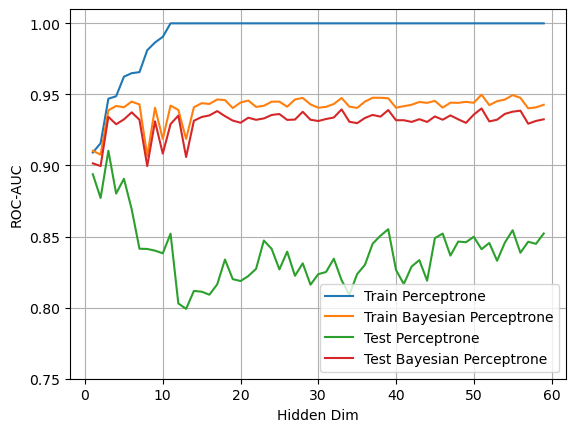
\includegraphics[width=1\linewidth]{roc_auc.png}
        \caption{Зависимость ROC--AUC от размерности скрытого состояния на тренировочных и тестовых данных}
        \label{fig:enter-label}
    \end{figure}

    \section{Выводы}
    По результатам работы можно сделать следующие выводы:
    \begin{itemize}
        \item с ростом сложности модели байесовская нейронная сеть не переобучилась;
        \item значение ROC-AUC на тестовой выборке имеет очень высокую корреляцию со значением ROC-AUC на тренировочной выборке (0.97 по Пирсону). Следовательно, для подбора гиперпараметров можно ориентироваться на метрики, полученные по тренировочной выборке. Это даёт нам возможность отказаться от деления на тренировочную и валидационную выборки для подбора гиперпараметров.
    \end{itemize}

    Так же стоит отметить, что данный подход переносится на другие архитектуры нейронных сетей (рекуррентные, свёрточные, трансформеры).

    Имплементация данного подхода была выполнена с использованием PyTorch. Весь исходный код для проведения экспериментов размещён по адресу \url{https://github.com/dimabasow/bayesian-neural-networks}.

\end{document}
